\documentclass[a4paper, 12pt]{article}

%\usepackage{cmap}
\usepackage[T2A]{fontenc}
\usepackage[utf8]{inputenc}
\usepackage[english, russian]{babel}
\usepackage{graphicx}
\usepackage[top=1in, bottom=1in, left=3.2cm, right=2.6cm]{geometry}
\graphicspath{./}
\usepackage{biblatex}
\addbibresource{lib.bib}
\linespread{1.5}
\usepackage{ragged2e}
\justifying
\usepackage{listings}
\usepackage{color}
\usepackage{amsmath}


\begin{document}
	
\begin{titlepage}
	\fontsize{12pt}{12pt}\selectfont
	\begin{figure}[t!]
		\centering
		
\includegraphics[scale=0.8]{bmstu}
	\end{figure}
	
	\noindent\rule{15cm}{3pt}
	\newline\newline
	\noindent 
	ФАКУЛЬТЕТ 
	\underline{«Информатика и системы управления»} \newline
	
	\noindent КАФЕДРА \underline{«Программное обеспечение ЭВМ и информационные технологии»}\newline\newline\newline\newline\newline
	
	\centering {\Large \textbf{Отчет по лабораторной работе № 6}}
	\vspace{4mm}
	
	\centering {\Large \textbf{По курсу:} Моделирование
		\vspace{8mm}}
	\\ \centering {\Large \textbf{На тему:} Моделирование работы кондитерской}
	\vspace{20mm}
	
	
	\begin{flushright}
		{\small	\textbf{Студент:}\\ Турсунов Жасурбек Рустамович \\ \textbf{Группа:} ИУ7-76Б
			\vspace{3mm}
			\\\textbf{Преподователь:} \\ Рудаков Игорь Владимирович }
	\end{flushright}
	
	\begin{center}
		\vfill
		Москва, \the\year
		~г.
	\end{center}
\end{titlepage}

\tableofcontents
\clearpage
\newpage


\section{{Задание}}

\hspace*{5mm} В кондитерскую приходят клиенты каждые $4\pm1$ минуты. Обслуживание на кассе просиходит $3\pm2$ минуты. Если в очередь на кассу содержит больше 5 человек, то клиент уходит. С вероятностью 10\% клиента не заинтересует ассортимент и он уйдет; 30\%~--- клиент закажет уже готовую продукцию, что приведёт к выдаче; 5\%~--- продукцию, которую по тем или иным причинам приготовить не представляется возможным, что приведёт к уходу клиента; 35\%~--- клиент закажет продукцию, которую будет необходимо и возможно приготовить. Заказ клиента с 60\% вероятностью будет маленьким, а с вероятностью 40\%~--- большим. Повар 1 и повар 2 занимаются только маленькими заказами, а повар 3~--- только большими. Время приготовления продукции каждым поваром составляет $10\pm2$ минут, $11\pm2$ минут и $20\pm4$ минут соотвественно. Выбор между поваром 1 и поваром 2 происходит по равномерному распределению. Результат приготовления попадает на выдачу. С вероятностью 5\% продукция на выдаче не понравится клиенту и он уйдёт.

Промоделировать процесс обслуживания 300 клиентов, определить вероятность отказа.
\\ \hspace*{5mm}На рисунке 1 изображена структурная схема рассматриваемой концептуальной модели
\begin{figure}[h!]
	\centering 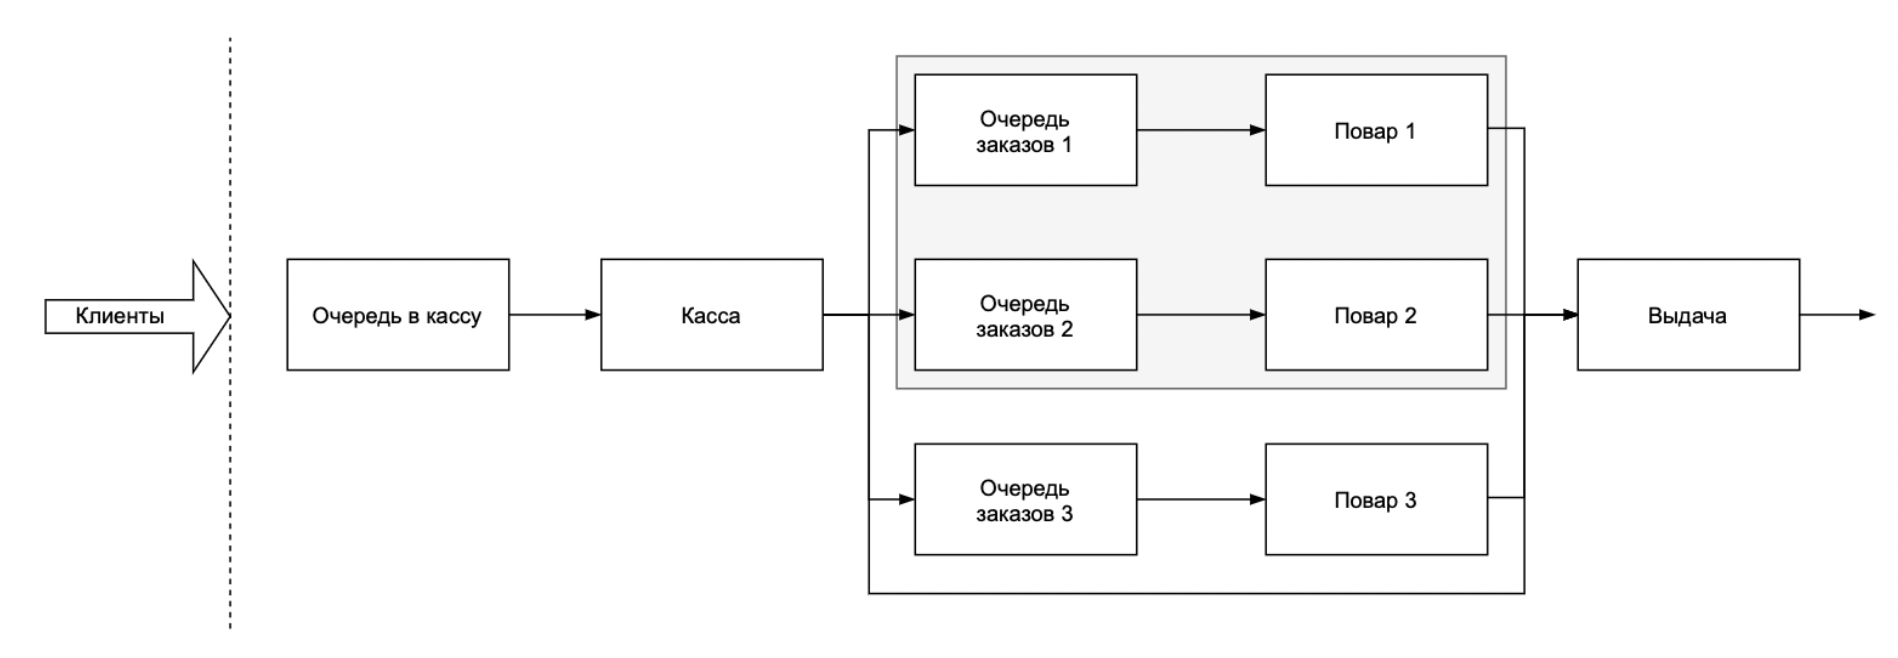
\includegraphics[scale=0.5]{schema}
\end{figure}

\clearpage
\newpage
\section{{Результаты}}
\hspace*{5mm}Так как вероятность отказа - это промежуток, поэтому прогоним модель 100 раз и найдем максимальное и минимальное значение. На рисунке 2 показаны результаты выполнения программы для 300 клиентов.
\begin{figure}[h!]
	\centering 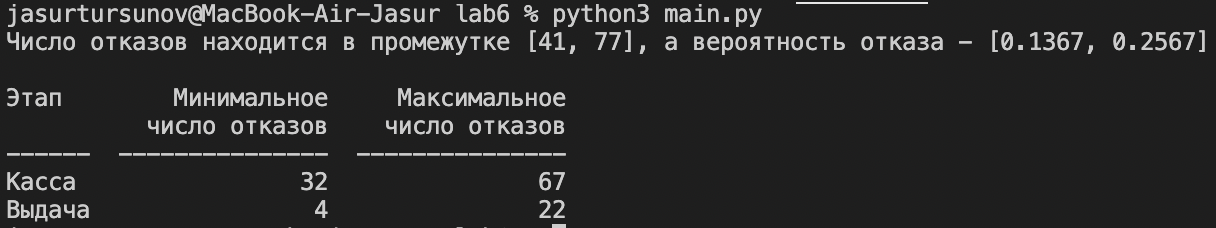
\includegraphics[scale=0.8]{300}
\end{figure}

\section{Листинг кода}
\definecolor{codegreen}{rgb}{0,0.6,0}
\definecolor{codegray}{rgb}{0.5,0.5,0.5}
\definecolor{codepurple}{rgb}{0.58,0,0.82}
\definecolor{backcolour}{rgb}{0.95,0.95,0.92}

\lstdefinestyle{mystyle}{
	backgroundcolor=\color{backcolour},   
	commentstyle=\color{codegreen},
	keywordstyle=\color{magenta},
	numberstyle=\tiny\color{codegray},
	stringstyle=\color{codepurple},
	basicstyle=\ttfamily\footnotesize,
	breakatwhitespace=false,         
	breaklines=false,                 
	captionpos=b,                    
	keepspaces=true,                 
	numbers=left,                    
	numbersep=5pt,                  
	showspaces=false,                
	showstringspaces=false,
	showtabs=false,                  
	tabsize=4
}

\lstset{style=mystyle}

\begin{lstlisting}[language=Python, caption = Программная реализация работы кондитерской]
def main():

	refusals_counters = []

	iterations_qty = 100

	transactions_qty = 300


	while iterations_qty := iterations_qty - 1:
	
		model = Model(TransactionGenerator(4, 1, 0, transactions_qty))

		
		cashier = Device("Cashbox", 3, 2, 5)


		cook1 = Device("chef 1", 10, 2, None)

		cook2 = Device("chef 2", 11, 2, None)

		cook3 = Device("chef 3", 20, 4, None)


		delivery = Device("Output", 1, 0.25, None)


		refusal = Device("Refuse", 0, 0, -1)

		success = Device("Succsess", 0, 0, -1)


		cashier.add_filled_transfer(1, refusal)

		cashier.add_post_transfer(0.1, refusal)

		cashier.add_post_transfer(0.4, delivery)

		cashier.add_post_transfer(0.05, refusal)

		cashier.add_post_transfer(0.45 * 0.6 / 2, cook1)

		cashier.add_post_transfer(0.45 * 0.6 / 2, cook2)

		cashier.add_post_transfer(0.45 * 0.4, cook3)


		cook1.add_post_transfer(1, delivery)

		cook2.add_post_transfer(1, delivery)

		cook3.add_post_transfer(1, delivery)


		delivery.add_post_transfer(0.05, refusal)

		delivery.add_post_transfer(0.95, success)


		model.pipeline += [

			cashier,

			cook1,

			cook2,

			cook3,

			delivery,

			]


		model.run()


		refusals_counters.append(refusal.income_counters.copy())


\end{lstlisting}
\end{document}